\documentclass[12pt]{article}

% Include some useful packages 
\usepackage[a4paper, margin = 1in, tmargin = 0.5in]{geometry} % Set the page and margin sizes for your document. 
% In this case I use a 1 inch margin in all sides except the top, which has a half in margin.
\usepackage{amsmath} % for an expanded list of mathematical symbols
\usepackage{float} % for help with placing figures right where I want them in the text. 
\usepackage{graphicx} % for importing pictures




% Begin Document
%==============================================================================
\begin{document}
% Information to automatically create a document header
\title{Sample Homework Submission - Stat 5100}
\author{Your Name}
\date{(Assignment Due Date)}
\maketitle

\section*{Problem 1}
\subsection*{Part a}
Notice how both ``Problem 1'' and ``Part a'' are listed on their own lines and bolded. This will be helpful to the grader as they navigate through your submission. This will also be helpful to you as you work on pieces of the homework throughout the week. With the exception of Homework 1, it is strongly recommended that you work on these assignments one piece at a time.

\subsection*{Part b}
Be sure to give every figure a caption and be sure to reference each figure in the text. This is a great way to determine which output is relevant and which is not: if you don’t have a need to reference the figure in the text, then it is probably not relevant for the submission. For example, Figure \ref{scatterfig} shows a nice looking set of scatterplots, while Figure \ref{mapfig} shows a nice looking map. Notice that the order of the figures matches the order in which I referenced them in the text.

\begin{figure}[H] % ``H'' tells latex to place the figure as close as it can in the text to where I have defined it. 
\center % center the figure in the page
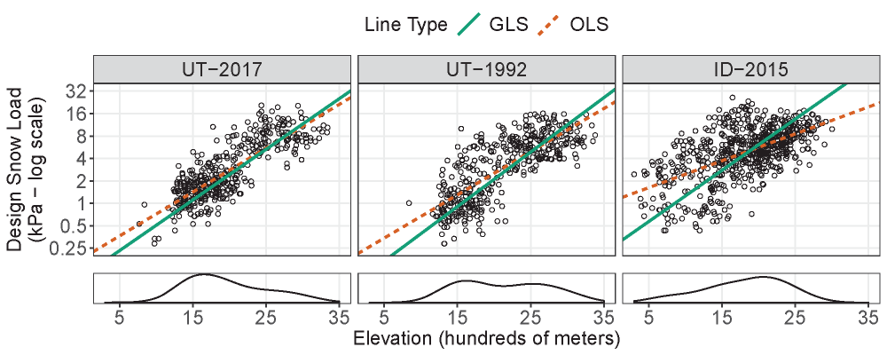
\includegraphics[width = 0.75\textwidth]{scatter1.png} % width=0.5\textwidth tells the program that the picture should span 75% of the page. 
\caption{Plots of elevation against design ground snow load (log scale) for three select datasets in the Northwest United States.}
\label{scatterfig}
\end{figure} 

\begin{figure}[H] 
\center 
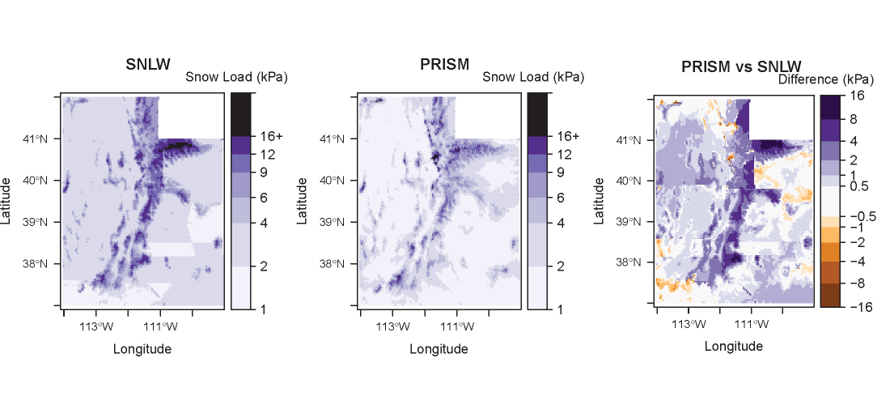
\includegraphics[width = 0.75\textwidth]{map1.png} 
\caption{Maps of design ground snow load predictions for Utah.}
\label{mapfig}
\end{figure} 
\newpage

\section*{Problem 2}
\subsection*{Part a}
Notice the large amount of white space between the end of Problem 1 and the start of Problem 2. This is because each problem needs to start on its own page. This would be a waste of space if you were printing the assignment, but remember that all assignments are submitted electronically. This separation is crucial for helping Jared navigate through each problem in the homework. 

\subsection*{Part b}
Should you choose not to answer a particular problem or problem part, it is courteous (though not required) to indicate this as shown in part c. 

\subsection*{Part c}
No answer

\subsection*{Part d}
Please post any questions about this homework sample on Piazza. Also be sure to continue scrolling to see the guidelines for the code appendix. 


\newpage
\section*{Appendix: SAS Code}

\subsection*{Problem 1 Code}
\begin{verbatim}
/* Complete SAS code for STAT 5100 Homework 1 */ 
/* Enter Data */
data reading;
	input Method $ CompChange @@;
	cards;
  Basal  1    Basal  1.5  Basal -2.5  Basal -2.5  Basal  -1    Basal  -5.5
  Basal -2.5  Basal -4.5  Basal  0    Basal -1    Basal  -2    Basal  -1.5
  Basal -3.5  Basal  1    Basal -2    Basal -0.5  Basal  -3.5  Basal  -3.5
  Basal -2.5  Basal -3.5  Basal -0.5  Basal  0    DRTA    2    DRTA   -1
  DRTA   0    DRTA   0.5  DRTA   -1.5 DRTA  -1    DRTA    2    DRTA    1.5
  DRTA  -0.5  DRTA  -1.5  DRTA   0    DRTA  -0.5  DRTA    2    DRTA   -0.5
  DRTA   1    DRTA   4.5  DRTA   2    DRTA  -1.5  DRTA    2.5  DRTA    0.5
  DRTA   1.5  DRTA   1
;
run;
/* Compare two groups */
proc ttest data=reading;
  class Method;
  var CompChange;
  title1 'Two-group comparison';
run;

\end{verbatim}


\subsection*{Problem 2 Code}
\begin{verbatim}
Place your SAS code for problem 2 in the verbatim environment. 

Be careful that the code does not extend off the page like this: (watch this code bleed off of the page..........)
\end{verbatim}

% End the Document
%==============================================================================
\end{document}